\documentclass[tikz,border=10pt]{standalone}
% no extra libraries needed for plain coordinates
\begin{document}
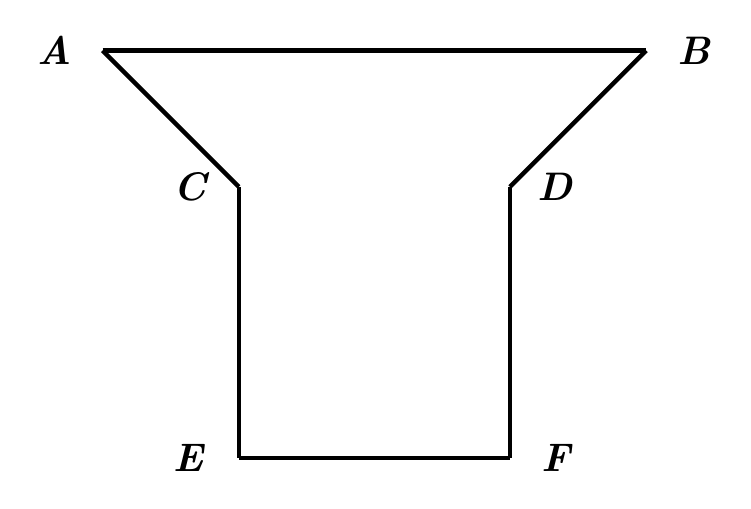
\begin{tikzpicture}[line join=round, line width=1.6pt, draw=black]
  % Scale s = 0.018223 cm/px, centred on ink bbox centre (257, 187.5)
  % x_t = (px-257)*s, y_t = (187.5-py)*s
  \coordinate (A) at (-3.462,2.596);
  \coordinate (B) at (3.444,2.596);
  \coordinate (C) at (-1.731,0.866);
  \coordinate (D) at (1.713,0.866);
  \coordinate (E) at (-1.731,-2.579);
  \coordinate (F) at (1.713,-2.579);

  % Outline: geometry and stroke width unchanged
  \draw (A) -- (B);
  \draw (A) -- (C);
  \draw (B) -- (D);
  \draw (C) -- (E);
  \draw (D) -- (F);
  \draw (E) -- (F);

  % Vertex labels: \Large, bold italic text; anchors unchanged
  % A, E left of vertex; B, F right; C left; D right
  \node[left=0.25cm, font=\Large] at (A) {\textbf{\textit{A}}};
  \node[right=0.25cm, font=\Large] at (B) {\textbf{\textit{B}}};
  \node[left=0.2cm, font=\Large] at (C) {\textbf{\textit{C}}};
  \node[right=0.2cm, font=\Large] at (D) {\textbf{\textit{D}}};
  \node[left=0.25cm, font=\Large] at (E) {\textbf{\textit{E}}};
  \node[right=0.25cm, font=\Large] at (F) {\textbf{\textit{F}}};
\end{tikzpicture}
\end{document}